%%%%%%%%%%%%%%%%%%%%%%%%%%%%%%%%%%%%%%%%%
% Journal Article
% LaTeX Template
% Version 1.4 (15/5/16)
%
% This template has been downloaded from:
% http://www.LaTeXTemplates.com
%
% Original author:
% Frits Wenneker (http://www.howtotex.com) with extensive modifications by
% Vel (vel@LaTeXTemplates.com)
%
% License:
% CC BY-NC-SA 3.0 (http://creativecommons.org/licenses/by-nc-sa/3.0/)
%
%%%%%%%%%%%%%%%%%%%%%%%%%%%%%%%%%%%%%%%%%

%----------------------------------------------------------------------------------------
%	PACKAGES AND OTHER DOCUMENT CONFIGURATIONS
%----------------------------------------------------------------------------------------

\documentclass[twoside,twocolumn,10.8pt]{article}

\usepackage{graphicx}

\usepackage[sc]{mathpazo} % Use the Palatino font
\usepackage[T1]{fontenc} % Use 8-bit encoding that has 256 glyphs
\linespread{1.05} % Line spacing - Palatino needs more space between lines
\usepackage{microtype} % Slightly tweak font spacing for aesthetics

\usepackage[english]{babel} % Language hyphenation and typographical rules

\usepackage[hmarginratio=1:1,top=32mm,columnsep=25pt, margin=0.85in]{geometry} % Document margins
\usepackage[hang, small,labelfont=bf,up,textfont=it,up, skip=1pt]{caption} % Custom captions under/above floats in tables or figures
\usepackage{booktabs} % Horizontal rules in tables

\usepackage{lettrine} % The lettrine is the first enlarged letter at the beginning of the text

\usepackage{enumitem} % Customized lists
\setlist[itemize]{noitemsep} % Make itemize lists more compact

\usepackage{abstract} % Allows abstract customization
\renewcommand{\abstractnamefont}{\normalfont\bfseries} % Set the "Abstract" text to bold
\renewcommand{\abstracttextfont}{\normalfont\small\itshape} % Set the abstract itself to small italic text

\usepackage{titlesec} % Allows customization of titles
\renewcommand\thesection{\Roman{section}} % Roman numerals for the sections
\renewcommand\thesubsection{\roman{subsection}} % roman numerals for subsections
\titleformat{\section}[block]{\large\scshape\centering}{\thesection.}{1em}{} % Change the look of the section titles
\titleformat{\subsection}[block]{\large}{\thesubsection.}{1em}{} % Change the look of the section titles

\usepackage{fancyhdr} % Headers and footers
\pagestyle{fancy} % All pages have headers and footers
\fancyhead{} % Blank out the default header
\fancyfoot{} % Blank out the default footer
\fancyhead[C]{COMP5329 Deep Learning$\bullet$ Assignment 2 $\bullet$ report} % Custom header text
\renewcommand{\headrulewidth}{1pt}
\fancyfoot[C]{\thepage} % Custom footer text

\usepackage{titling} % Customizing the title section

\usepackage{hyperref} % For hyperlinks in the PDF

%----------------------------------------------------------------------------------------
%	TITLE SECTION
%----------------------------------------------------------------------------------------

\setlength{\droptitle}{-4\baselineskip} % Move the title up
\setlength{\parskip}{0.5em}

\pretitle{\begin{center}\Huge\bfseries} % Article title formatting
\posttitle{\end{center}} % Article title closing formatting
\title{COMP5329 Assingment2} % Article title
\usepackage{authblk}
\author[1]{Dongdong Zhang}
\author[2]{Quan Chen}
\author[3]{Rui Wang}

\affil[1,2,3]{University of Sydney}
{	
    \makeatletter
    \renewcommand\AB@affilsepx{: \protect\Affilfont}
    \makeatother

    \affil[ ]{Student ID}

    \makeatletter
    \renewcommand\AB@affilsepx{, \protect\Affilfont}
    \makeatother

    \affil[1]{470161133}
    \affil[2]{470199228}
    \affil[3]{470208162}
}


\date{\today} % Leave empty to omit a date
\renewcommand{\maketitlehookd}{%
\begin{abstract}
Computer vision has always been a trending filed in deep learning. The main problem in this area is to classify patterns into different classes. Traditional approaches of machine learning such as k-nearest neighbors can be utilized to address this problem. However, this requires preprocessing of images and transform them into matrices.  In addition to these methods, multilayer neural networks as a deep learning approach can also be applied   to address the classification problem. When convolutional neural network was utilized in computer vision, the accuracy of classification was improved dramatically. In this project, we propose a convolutional neural network with some other techniques to address an image classification problem. The dataset includes all the images of numbers from 0 to 9 and the alphabet letters from A to Z including both lower-case and upper-case letters.   
\end{abstract}
}

%----------------------------------------------------------------------------------------

\begin{document}

% Print the title
\maketitle

%----------------------------------------------------------------------------------------
%	ARTICLE CONTENTS
%----------------------------------------------------------------------------------------

\section{Introduction}

\lettrine[nindent=0em,lines=3]{C}{}lassifying images of different classes has always been a trending problem in deep learning. This problem requires a discrimination of images among many classes. It is important because it can be applied in many fields. For instance, face recognition can be utilized in public security. it can also help classify disease in medical industry. All of these applications require a mass of images as input and then classify the images into several classes. Convolutional neural network has drawn extensive attention on computer vision classification since it produces state-of-art performance. The classification using convolutional neural network has been proved to be extremely effective computer vision. Today, most of the framework relies on powerful convolutional neural network \cite{R1}.. Therefore, it is important to understand how to classify images using convolutional neural network. 


\noindent In this project, we propose a convolutional neural network to finish a multi-class classification problem. Meanwhile, the shift, rotation and scaling of data augmentation are also utilized in this project.

\noindent The rest of the report is organized as follows. Section 2 reviews the related work on image classification. Section 3 introduces techniques. Section 4 describes the experiment and the results, followed by discussions and conclusions in section 5.

%------------------------------------------------

\section{Related work}

Image classification has always been a trending problem in deep learning. Many approaches have been utilized to address this problem. Traditional machine learning algorithms such as support vector machine, k-nearest neighbors and Naïve-Bayes classifier can be utilized to address this problem. Preprocessing might be necessary to transform the image into data matrix. A remarkable convolutional neural network was proposed in 2012, typically known as AlexNet [1]. It utilized 5 convolutional layers and 3 fully connected layers and got state-of-art results at that time. In 2015, another milestone network known as VGG was created \cite {R2}. This is one of the most commonly used convolutional neural network.
% \begin{itemize}
% \item Donec dolor arcu, rutrum id molestie in, viverra sed diam
% \item Curabitur feugiat
% \item turpis sed auctor facilisis
% \item arcu eros accumsan lorem, at posuere mi diam sit amet tortor
% \item Fusce fermentum, mi sit amet euismod rutrum
% \item sem lorem molestie diam, iaculis aliquet sapien tortor non nisi
% \item Pellentesque bibendum pretium aliquet
% \end{itemize}
% \blindtext % Dummy text

% Text requiring further explanation\footnote{Example footnote}.

%------------------------------------------------

\section{Technique}

In this section, we will introduce the proposed structure of the convolutional neural network as well as other techniques used on it. To explain the structure of the network, we assume the input image to be \bf X \rm. 
% \begin{table}
% \caption{Example table}
% \centering
% \begin{tabular}{llr}
% \toprule
% \multicolumn{2}{c}{Name} \\
% \cmidrule(r){1-2}
% First name & Last Name & Grade \\
% \midrule
% John & Doe & $7.5$ \\
% Richard & Miles & $2$ \\
% \bottomrule
% \end{tabular}
% \end{table}

\subsection{Convolutional neural network}
The modules of a convolutional neural network usually are convolutional layer, pooling layer and fully connected layer. Convolutional layer assigns a convolution operation to the input image. More specifically, filters with some size (usually 2x2) are used to extract features. Pooling layer can extract the combination of outputs of neurons at on layer to into a single neuron in the next layer. For instance, max pooling takes the maximum value of the neurons of a cluster from prior layer. Fully connected layer can connect the neurons from one layer to the neurons in another layer. in our design, it has the same function as dense layer. 

\noindent Given the input data X, we feed it into a convolutional neural network as the input layer. The structure of the whole network is shown in Figure 1. As the figure indicates, the network utilizes two convolutional layers and max pooling layers. Then the output is fed into dropout layer to avoid overfitting. Next, densely connected layers are utilized to get the final output.

\begin{figure}[h]
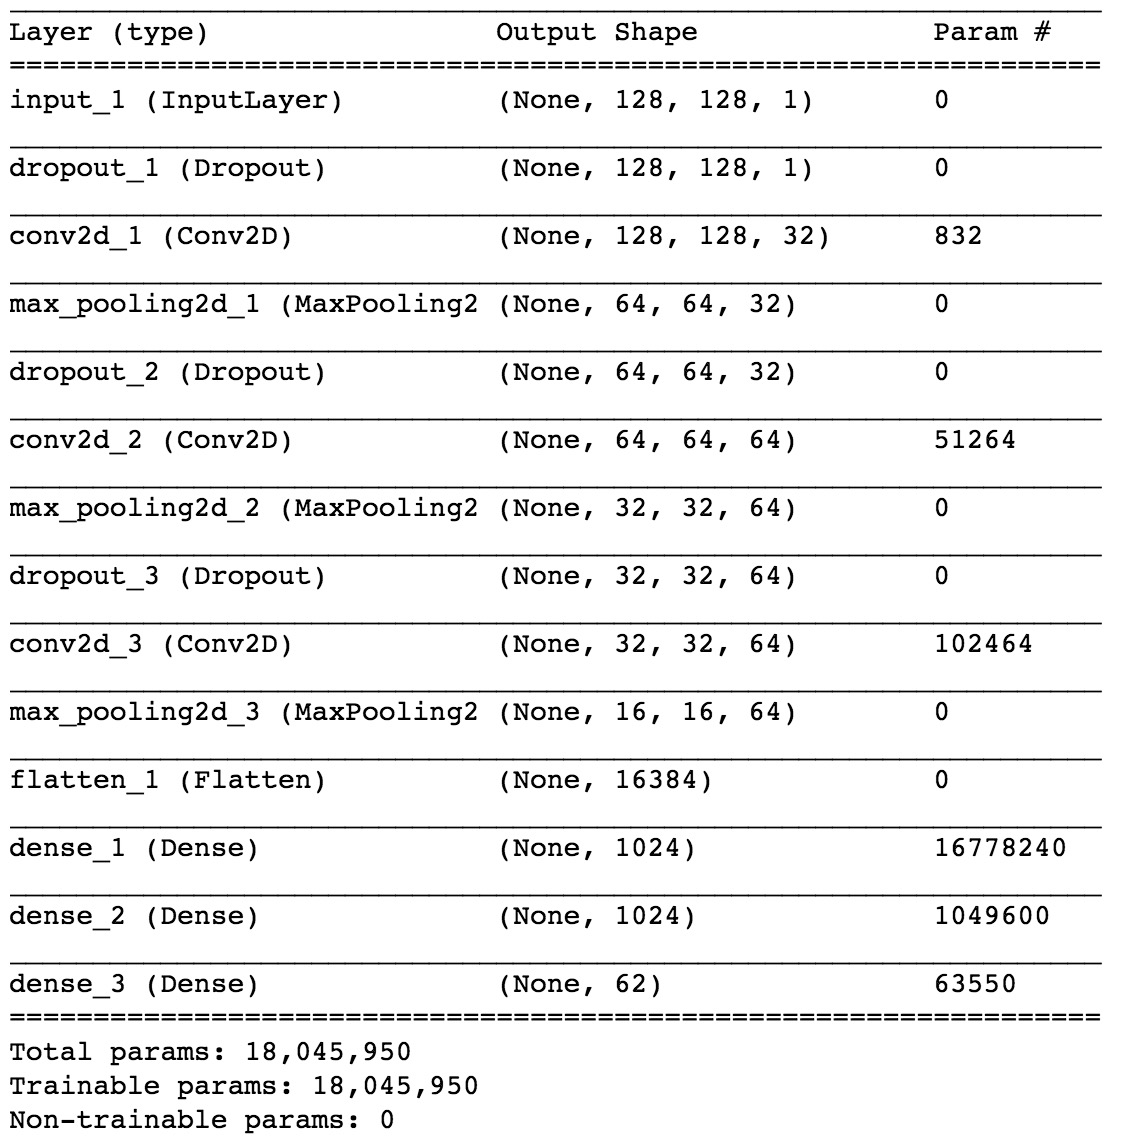
\includegraphics[width=8cm]{model_detail.png}
\centering
\caption{Model detail}\label{fig1}
\end{figure}


\subsection{Activation function}

In this design, the activation functions are applied. 
ReLU activation function is an extensively used activation function in machine learning. It is defined as 
\begin{equation}
\label{eq:1}
f(x) = max(0,x)
\end{equation}

\noindent where $max(0,x)$ indicates the maximum value between 0 and x. ReLU function is one sided and can be used to avoid gradient vanishing problem where at some point, the gradient of the activation function becomes 0. Nevertheless, ReLU function indicates that the negative values of input are treated as 0s, which means some neurons will be dead. In our design, ReLU is chosen as the in the convolutional layers. \cite{R3}
%------------------------------------------------

\subsection{Softmax and cross entropy loss}

Before the output layer of the network, softmax function is utilized to assign conditional probabilities to each one of 
the target classes. The one with highest probability indicates the resulted label for the input data. The function can be expressed as 

\begin{equation}
\label{eq:2}
\widehat{P}(class_{k}|x)=\frac{e^{net_k}}{\sum_{i=1}^{K}e^{net_i}}
\end{equation}

\noindent where $\sum_{i=1}^{d}x_iw_{ji}+b_j$, which is the input to the activation function. K indicates the total number of $net_k$. In reality, there will be some differences between the output \bf z \rm and the ground-truth \bf t \rm. To measure these errors and optimize the network, loss functions are defined. Typically, the Euclidean distance between \bf t \rm and \bf z \rm is chosen as the loss function. In practice, we discovered that cross-entropy function 

\begin{equation}
\label{eq:3}
J(\mathbf{t,z})=-\sum_{k=1}^{C}t_klog(z_k)
\end{equation}

\noindent results a better performance. \cite{R3}

\subsection{Adam}

In this project, we use Adam as our optimizer.  This optimization method uses the averages of both gradients and the second moments of gradients. The update of Adam is given by: 

\begin{equation}
\label{eq:4}
\theta _{t+1}=\theta_{t+1}+\frac{\eta}{\sqrt{\hat{v}+\epsilon }}\widehat{m_t}
\end{equation}

\begin{equation}
\label{eq:5}
\widehat{m_t}=\frac{m_t}{1-\beta_1^t},\ \widehat{v_t}=\frac{v_t}{1-\beta_2^t}
\end{equation}

\begin{equation}
\label{eq:6}
m_t=\beta_1m_{t-1}+(1-\beta_1)g_t
\end{equation}

\begin{equation}
\label{eq:7}
v_t=\beta_2v_{t-1}+(1-\beta_2)g_t^2
\end{equation}

\noindent where $\epsilon$ is a small scalar to avoid division by 0, and $\beta_1$ and $\beta_2$ are the forgetting factors of the gradients and the second moments of gradients. 

\subsection{Dropout}

Overfitting is a common issue in deep learning. This problem means that the neural network could be overfitting with one dataset; once the data is changed, the accuracy of this network could decrease significantly. Dropout process sets some neurons of the network to be zero. In this case, equation (1) can be rewritten as 

\begin{equation}
\label{eq:8}
y_j=f((\sum_{i=1}^{d}x_iw_{ji})r_j+b_j)
\end{equation}

\noindent where $r_j$ represents the Bernoulli random variable with probability p. \cite{R3}

\subsection{Weight decay}

This module is applied to address two problems: firstly, it can choose the minimum weight vector to avoid irrelevant components; secondly, it can reduce some of the static noise on the targets \cite{R4}. This can be achieved by adding penalization to large weights \cite{R3}:

\begin{equation}
\label{eq:9}
\mathcal{L}_{new}(\textbf{w})=\mathcal{L}_{old}(\textbf{w})+\frac{1}{2}\lambda\sum_{i}w_i^2
\end{equation}


\subsection{Data augmentation}

Data augmentation is a technique that can be utilized to reduce the effect of overfitting and increase the number of training data. There are several ways of processing data in data augmentation. In this project, we choose shifting, rotation and scaling as our approaches for image augmentation. All the images in the dataset are processed by augmentation. We shift the images away from their original position by 5\%. The direction of shifting is randomly chosen. The images are rotated by 12 degrees. The direction of rotation is random. We also amplify or shrink the image by 5\% scaling. This technique is essential for boosting the performance of the network. The data size is increased because each image has three similar images which are shifted, rotated, zoomed in or zoomed out. This approach can also avoid the effect of overfitting since it increases the variety of the input dataset. This helps to increase the accuracy of validation. 

\section{Experiments and results}

The dataset we utilized are images folder files that contain train-set folder within 37,883 png items, vali-set folder within 6,263 png items, and .txt files of their labels. There are 62 corresponding classes for this dataset. It contains ten roman numerals and twenty-six English letters  with upper-case and lower-case. Overall, training data is 37,883 png files with their labels, and validating data is 6,263 png files with their labels. Before implementation, the data is randomly sorted. The experiments are implemented in python3.6 running on a Ubuntu18 LTS 1080Ti, keras 2.1.6 with tensorflow-gpu backend.The total training time will be approximately 90 minutes. 

\subsection{Result}



\begin{figure}[h]
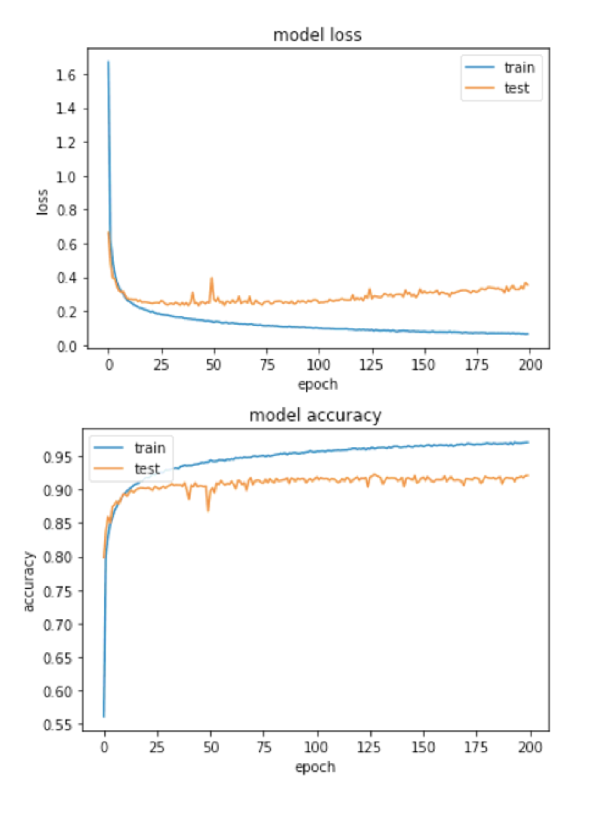
\includegraphics[width=8cm]{acc_loss.png}
\caption{Loss and Accuracy trend}\label{fig2}
\centering
\end{figure}


% \begin{figure}[h]
% 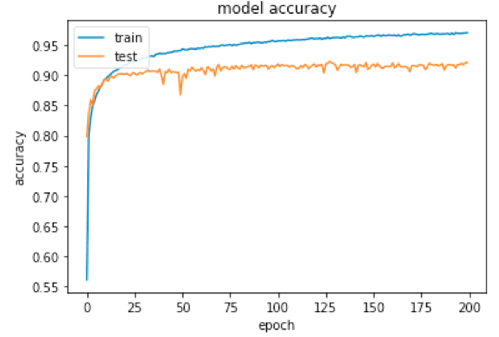
\includegraphics[width=8cm]{model_acc.png}
% \centering
% \caption{Figure captionxxxxxxxxxxxxxxxxxx}\label{fig2}
% \end{figure}


\noindent Our best accuracy is 92.13\% which means 493 predictions are wrong. The parameters we use is 5e-4, drop rate is 0.3, 0.2, 0.1. Rotation\_range = 12, width\_shift\_range = 0.05, height\_shift\_range = 0.05, zoom\_range = 0.05. Batch size is 256, 200 epochs.


\noindent Through this experiment, we develop cross entropy and softmax loss, dropout, weight decay, augmentation and batch normalization.


\noindent Since the labels are English letters and roman numerals, there are 62 classes, we translate it to one-hot representation. In those whole process, we applied idea --> code --> experiment cycle to make all experiment and make table to record each result in order to adjust parameters. 
We select train-set folder png files for training data, and vali-set folder png files for testing data. There are experiment detailed results and analysis below:

\subsection{Extensive analysis}


\subsubsection{Data augmentation analysis}


\begin{table*}[h]
\caption{Comparsion of different parameters}
\centering
\begin{tabular}{c c c c c c}
\hline
Data augmentation & Learning rate & Learning rate decay & Epoch & RT,WS,HS,ZR & Accuracy\\
\hline
F & 0.0005 & F & 60 & 10, 0.03, 0.03, 0.01 & 90.36\% \\
T & 0.0005 & F & 60 & 10, 0.03, 0.03, 0.01 & 91.36\% \\
T & 0.0005 & F & 80 & 12, 0.05, 0.05, 0.05 & 91.60\% \\
T & 0.0005 & T & 200 & 12, 0.05, 0.05, 0.05 & 92.13\% \\
\hline
\end{tabular}

RT = Rotation range, WS = Width shift, HS = Hight shift , ZR = Zoom rate
Batch size is 256

\label{table:1}
\end{table*}

In this experiment, we use data augmentation to increase the train data, This is essential for training because it can avoid overfitting in original train data and generalise it to the real word. Rotation, shift (height and width) and scaling is used to create more train images, the comparision table as Table 1. 


\noindent Rotation is important due to some of images’ character is italic and is not on the center. When we use this function in our model, accuracy will improve at least 1\% when using same epochs. 


\noindent When using data augmentation, in the first epoch we can get 80\% accuracy for validation data while the average score in our batch train data is around30\%. The reason is that data augmentation add more images to train data and more features need to be learned. After closing data augmentation  methods, the train accuracy and validation accuracy is close. Validation accuracy is small than train accuracy. 



\subsubsection{Learning decay analysis}
Without Learning decay in Adam, validation accuracy will improve quickly and oscillation heavily around 89\% accuracy. By using Learning decay, the validation accuracy line is more smooth and can achieve a better result.

\subsubsection{Feature-wise standard normalisation analysis}
When use Feature-wise standard normalisation, we find the accuracy is around 2\% and cannot come to convergence. This is not applied because the pixel is 0 and 1 because it will lose the essential and original information of train image. Rotation range is set to 12 and it cannot be lager due to the chapter is sensitive for angle and flip. We have set flip and rotation parameter to 40 and find accuracy cannot come to convergence. 


\subsubsection{Confusion matrix analysis}

\begin{figure}[h]
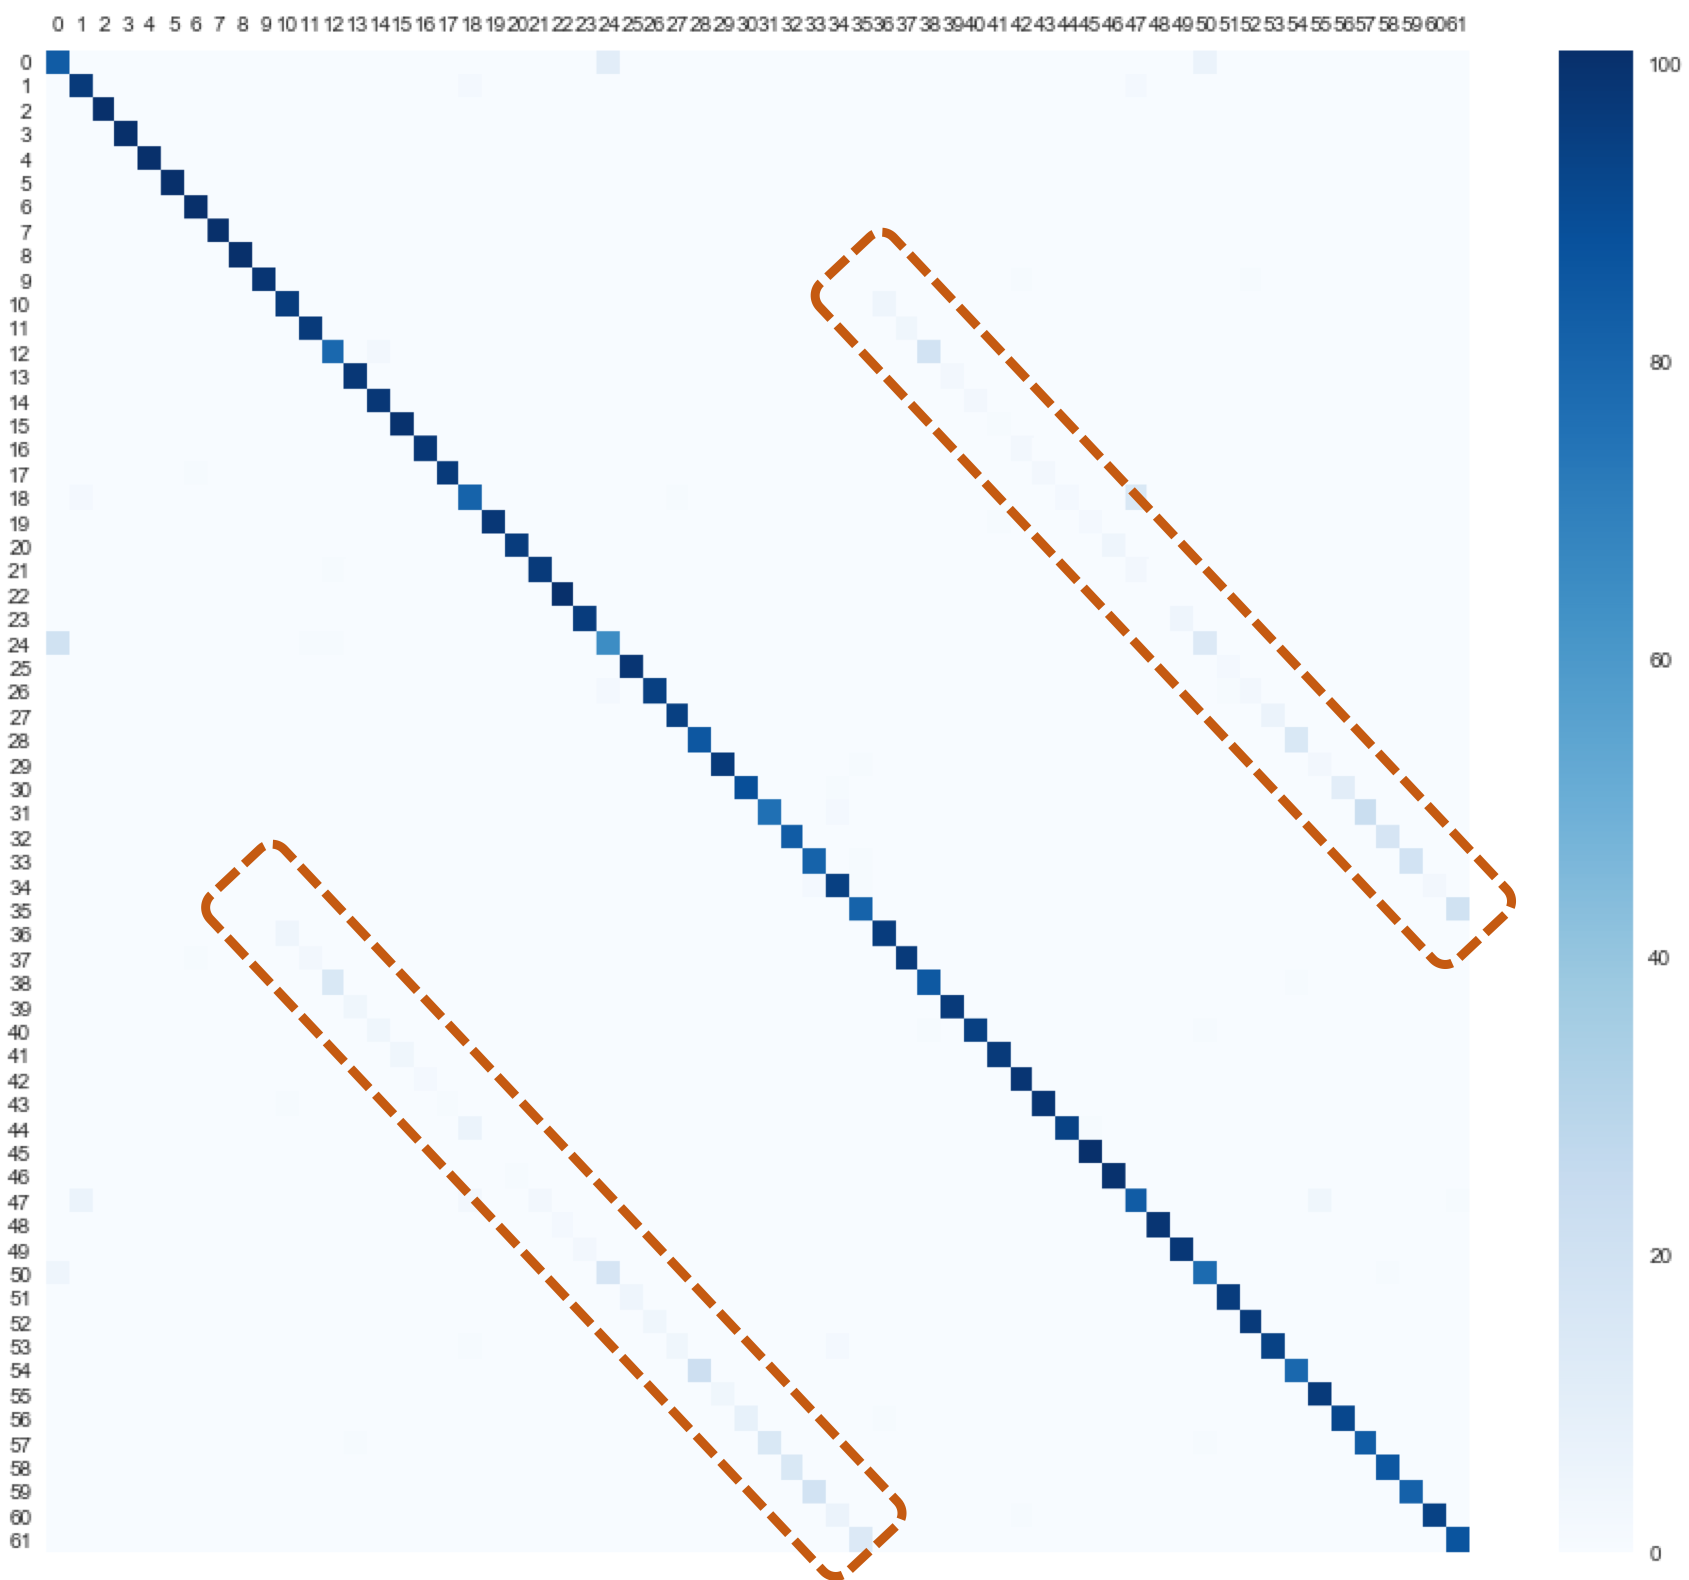
\includegraphics[width=8cm]{confusion_matrix.png}
\centering
\caption{Confusion Matrix}\label{fig3}
\end{figure}

\noindent By predicting the validation image and comparing the result with true label in confusion matrix, it is easy to find diagonal line across the whole diagram. From the whole Confusion Matrix we can see the middle line’s colour is deep and other lines are light. It shows our model do well in predictions to some extend. The upper and lower line is symmetrical and intuitive, it shows that our model’s error mainly comes from wrongly prediction between lowercase and uppercase of one character. Some of the outlier points which not located in those three line shows the second error comes from the wrongly prediction between number and character (such as ‘1’ and ‘I’).

\subsubsection{Wrong prediction analysis}

\begin{figure}[h]
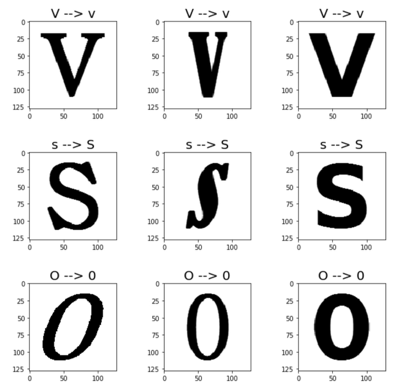
\includegraphics[width=8cm]{wront_pic_ana.png}
\centering
\caption{Wrong predict example}\label{fig4}
\end{figure}

\begin{table}[h]
\caption{Wrong predict example count}
\centering
\begin{tabular}{c|c}
\hline
RealLabel—>WrongLabel & Count\\
\hline
V—>v & 23 \\
s—>S & 22 \\
O—>0(number) & 20 \\
Z—>z & 20 \\
C—>c & 19 \\
X—>x & 19 \\
x—>X & 19 \\
W—>w & 17 \\
o—>O & 17 \\
I—>l(lower L) & 15 \\
S—>s & 15 \\
c—>C & 15 \\
v—>V & 15 \\
\hline
\end{tabular}
\label{table:1}
\end{table}

\noindent We have counted the wrong prediction for our system. From some of the predicted label and true label with correspond to the image, we find some of image is really weird. Pleas look at Figure 4 and Table 2:

\subsubsection{Upper and lower character}

Such as o->O, V->v, s->S, Z->z, C->c, X->x etc. It's really hard to discriminate those pictures for our system. Zoom methods will be reconsidered carefully. 

\subsubsection{Number and character}

\noindent Number ‘0’ and character ‘O’, number ‘9’ and character ‘q’, number ‘1’ and character ‘I’ and ‘i’ is really hard to discriminate.

\noindent We checked some of the most wrong predicted label and find it is very hard to distinguish them even by human. Maybe this can be solved to develop more deep neural network to capture more details.

\subsubsection{Improvement}

We have check the wrong predict picture for those wrong predictions and find our next research will care more on how to discriminate those character and number. Some methods like scaling (Data augmentation) will be carefully considered because it might make our model harder to distinguish those characters.


\section{Discussion and conclusion}
\subsection{Discussions}

During our work on the image classification, we experienced the process of building convolutional neural network to classify images. Before doing this project, we only learned the big picture of image classification from lectures. We learned the basic principles of convolutional layer, pooling layer and fully connected layer. This project helps us to implement the network and classify real world dataset. Augmentation technique is applied for the first time in our assignment to boost the performance of the network.

\noindent We all consider our project to be a successful project. The entire procedure of implementation gives us the insight of how to build a convolutional neural network and why it is one of the most cutting-edge technique in image classification.

\subsection{Conclusions}
\noindent In this assignment we propose three convolutional layer, two max pooling layer, dropout layer with three dense layer for image multi-callsification task model.

\noindent By applying data augmentation, this model got 92.13\% accuracy. After analysis the wrong predicted example, we found we model’s defect which is can not to distinguish some of the uppercase and lowercase format of one character. Some of the number and character such as number ‘9’ and character ’q’ is also has higher wrong index. Next step we will concentrate more on those wrong predicted label and analysis it’s inartistic details. We might develop a more complex CNN structure in order to better to capture those details. LSTM and more data context will be considered more so the model can be capture enough details for each image.







% A statement requiring citation \cite{Figueredo:2009dg}.


% \blindtext % Dummy text

% \subsection{Subsection Two}

% \blindtext % Dummy text

%----------------------------------------------------------------------------------------
%	REFERENCE LIST
%----------------------------------------------------------------------------------------

\begin{thebibliography}{99} % Bibliography - this is intentionally simple in this template

\bibitem [1]{R1}
A. Krizhevsky, I. Sutskever, and G. E. Hinton. Imagenet classification with deep convolutional neural networks. In NIPS, pages 1106–1114, 2012.
\bibitem [2]{R2}
K. Simonyan and A. Zisserman. Very deep convolutional networks for large-scale image recognition. In ICLR, pages 1409–1556, 2015.
\bibitem [3]{R3}
D. Zhang, Q. Chen and R. Wang. Deep learning assignment 1 of the University of Sydney. 2018.
\bibitem [4]{R4}
A. Krough and J. Hertz. A Simple Weight Decay Can Improve Generalization. In NIPS, 1991.
 
\end{thebibliography}

%----------------------------------------------------------------------------------------

\end{document}
